\documentclass[11pt]{article}

% Load packages
\usepackage{minted}
\usepackage{amsmath, amsfonts, mathtools} % for math
\usepackage{graphicx, float} % for figures
\usepackage[margin=1in]{geometry} % to set margins
\usepackage{tcolorbox} % to create nice boxes
\tcbuselibrary{skins,breakable} % extra libraries for the nice boxes
\allowdisplaybreaks % allow aligned equations to display across pages

% Sets the default font to sans serif
% \renewcommand\familydefault{\sfdefault}

% Define a custom box for the solutions. Don't change this!
\newtcolorbox[]{solution}
    {colframe=red!20, 
        colback=white, 
        sharp corners,
        title=Solution,
        enhanced,
        breakable,
        coltitle=black,
        fonttitle=\bfseries,
        attach boxed title to top left={yshift*=-\tcboxedtitleheight/2, xshift=3mm},
        boxed title style={sharp corners, colback=red!20}
        }

\usepackage{boondox-calo}
\newcommand{\lr}[1]{\left(#1\right)}

\usepackage{hyperref}
\hypersetup{
    colorlinks=true,
    linkcolor=blue,
    filecolor=magenta,      
    urlcolor=cyan
}



% Write the document
\begin{document}
    \title{Extreme Computing: Homework 1}
    \author{Michael S. Emanuel, Jonathan Guillotte-Blouin, Erick Ruiz, Yue Sun}
    \date{February 25, 2019}
    \maketitle
    
  \section{Problem 1:  Couette Flow}
    % Problem statement
    Couette flow is a classic, basic flow pattern in which a fluid is confined between two, smooth parallel plates. The bottom plate (at $y=-h$) is stationary, while the top plate (at $y=h$) is moving with a constant velocity $U$. It is assumed that the flow is steady, fully developed, two-dimensional (i.e. independent of $z$), and there is a zero pressure gradient. Figure~\ref{fig:couette} shows a diagram of the flow configuration.
    \begin{figure}[H]
    	\centering
    	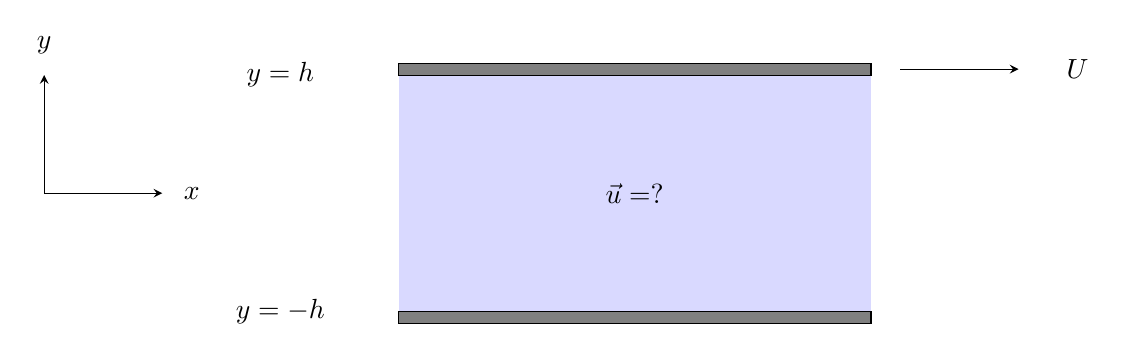
\begin{tikzpicture}[scale=1.5]
    		% fluid
    		\path[fill=blue!15!] (0,0) rectangle (4,2);
    		
    		% plates
    		\draw[fill=gray] (0,0) rectangle (4,-0.1);
    		\draw[fill=gray] (0,2) rectangle (4,2.1);
    		
    		% plate heights
    		\node at (-1,0) {$y=-h$};
    		\node at (-1,2) {$y=h$};
    		
    		% top plate velocity
    		\draw[->, >=stealth] (4.25,2.05) -- (5.25,2.05);
    		\node at (5.75,2.05) {$U$};
    		
    		% reference frame
    		\draw[<->, >=stealth] (-3,2) -- (-3,1) -- (-2,1);
    		\node at (-3,2.25) {$y$};
    		\node at (-1.75,1) {$x$};
    		
    		% velocity field
    		\node at (2,1) {$\vec{u} = $?};
    	\end{tikzpicture}
    	\caption{A schematic of the Couette flow configuration, with the velocity profile included.}
    	\label{fig:couette}
    \end{figure}
    Use no-slip boundary conditions to calculate the velocity and vorticity fields, the components of the shear stress tensor, the volume flow rate, and the average and maximum velocities in the channel. Also, make a plot of the velocity profile at a few different values of $U$. Be sure to put $y$ on the $y$-axis and $u(y)$ on the $x$-axis of your plot.

    % Solution    
    \begin{solution}
        % Problem 2 Solution
Let us start with the Navier-Stokes equations for an incompressible fluid.
\begin{align}
    \frac{\partial \vec{u}}{\partial t} + (\vec{u}\cdot\vec{\nabla})\vec{u} &= -\frac{1}{\rho}\vec{\nabla}p + \frac{\mu}{\rho}\nabla^2\vec{u} + \vec{f}\\
    \vec{\nabla}\cdot\vec{u} &= 0
\end{align}
Assuming that the external body forces acting on the fluid are negligible allows us to omit the last term on the right-hand side of the momentum equation.
\begin{equation}
    \frac{\partial \vec{u}}{\partial t} + (\vec{u}\cdot\vec{\nabla})\vec{u} = -\frac{1}{\rho}\vec{\nabla}p + \frac{\mu}{\rho}\nabla^2\vec{u}
    \label{nsm}
\end{equation}
Also, under the steady, fully developed flow assumption, the total time derivative can be taken as zero.
\begin{equation}
    \frac{d\vec{u}}{dt} = \frac{\partial \vec{u}}{\partial t} + (\vec{u}\cdot\vec{\nabla})\vec{u} = 0
\end{equation}
Furthermore, if the pressure gradient is zero, we can drop the first term on the right-hand side of equation (\ref{nsm}), which allows us to write the simplified momentum equation as 
\begin{equation}
    \nu\nabla^2\vec{u} = 0,
\end{equation}
where $\nu = \mu/\rho$ is the kinematic viscosity. Notice that we may rewrite the last equation as 
\begin{equation}
    \nabla^2\vec{u} = 0
\end{equation}
since it is understood that the kinematic viscosity is non-zero. 

Now, we are also told that the flow is two-dimensional, and since it is assumed that the flow does not vary along $x$, we may write $\vec{u} = u(y)\ \hat{x}$. Notice that we have concluded that $u=u(y)$, which allows us to write a single ordinary differential equation for $u(y)$.
\begin{equation}
    \frac{d^2u}{dy^2} = 0
    \label{odeu}
\end{equation}
We can then solve equation (\ref{odeu}) by direct integration to obtain the following solution.
\begin{equation}
    u(y) = c_1 y + c_2
\end{equation}
At this point, we must apply the boundary conditions. Remember that we are working with no-slip boundary conditions, which implies that $u(h)=U$ and $u(-h)=0$.
\begin{align}
    u(-h) &= 0 = -c_1 h + c_2 \label{bct}\\
    u(h) &= U = c_1 h + c_2 \label{bcb}
\end{align}
Solving equations (\ref{bct}) and (\ref{bcb}) simultaneously for $c_1$ and $c_2$ yields $c_1 = U/2h$ and $c_2 = U/2$. Thus, the velocity field for this particular geometry is
\begin{equation}
    \boxed{\vec{u} = \frac{U}{2}\left(\frac{y}{h}+1\right)\ \hat{x}.}
\end{equation}
Once we have the velocity field, it is straightforward to obtain the remaining relevant quantities. Let us start with the vorticity field, which we obtain by simply taking the curl of the velocity field.
\begin{equation}
    \boxed{\vec{\omega} = \vec{\nabla}\times\vec{u} = -\frac{U}{2h}\ \hat{z}}
\end{equation}
We now turn our attention to the shear stress. First, recall that the components of the stress tensor for an incompressible fluid may be written as follows.
\begin{equation}
    \sigma_{ik} = -p\delta_{ik} + \mu\left(\frac{\partial v_k}{\partial x_i} + \frac{\partial v_i}{\partial x_k}\right)
\end{equation}
Notice that the stress tensor is symmetric, and since we are only interested in the shear stress, we only need to calculate the off-diagonal elements. 
\begin{equation}
    \tau_{ik} = \mu\left(\frac{\partial v_k}{\partial x_i} + \frac{\partial v_i}{\partial x_k}\right)
\end{equation}
Most of these will be zero because only the $x$-component of our velocity field is non-zero. 
\begin{align}
    \tau_{xy} &= \tau_{yx} = \mu\frac{U}{2h}\\
    \tau_{yz} &= \tau_{zy} = 0\\
    \tau_{zx} &= \tau_{zx} = 0 
\end{align}
For compactness, we may write the end result in matrix form as follows.
\begin{equation}
    \boxed{\hat{\tau} 
    = 
    \begin{pmatrix}
        0 & \mu\frac{U}{2h} & 0\\
        \mu\frac{U}{2h} & 0 & 0\\
        0 & 0 & 0	
    \end{pmatrix}}
\end{equation}
To obtain the volume flow rate, we simply integrate the velocity field with respect to $y$ from $y=-h$ to $y=h$. 
\begin{equation}
    \boxed{Q = \int_{-h}^{h} \frac{U}{2}\left(\frac{y}{h}+1\right)\ dy = Uh}
\end{equation}
Finally, we calculate the maximum and average velocities. To do this, we note that the minimum and maximum velocities are at $y=-h$ and $y=h$, respectively. By inspection, the minimum velocity must be zero to obey the boundary condition at $y = -h$. Likewise, the maximum velocity must be $U_\text{max} = U$ to obey the boundary condition at $y = h$. Thus, we can calculate the average velocity as follows.
\begin{equation}
    \boxed{U_\text{avg} = \frac{U(h)+U(-h)}{2} = \frac{U}{2}}
\end{equation}

\begin{figure}[H]
	\centering
	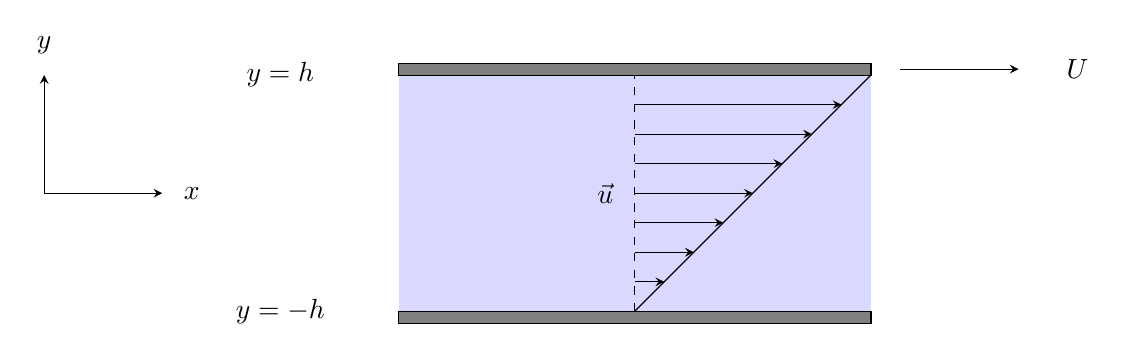
\begin{tikzpicture}[scale=1.5]
		% fluid
		\path[fill=blue!15!] (0,0) rectangle (4,2);
		
		% plates
		\draw[fill=gray] (0,0) rectangle (4,-0.1);
		\draw[fill=gray] (0,2) rectangle (4,2.1);
		
		% plate heights
		\node at (-1,0) {$y=-h$};
		\node at (-1,2) {$y=h$};
		
		% top plate velocity
		\draw[->, >=stealth] (4.25,2.05) -- (5.25,2.05);
		\node at (5.75,2.05) {$U$};
		
		% reference frame
		\draw[<->, >=stealth] (-3,2) -- (-3,1) -- (-2,1);
		\node at (-3,2.25) {$y$};
		\node at (-1.75,1) {$x$};
		
		% velocity field (jonathan's figure)
		\node at (1.75,1) {$\vec{u}$};
		\draw[dashed] (2,0) -- (2,2);
		\draw (2,0) -- (4,2);
		\foreach \x in {0.25,0.5,...,1.75}{
		    \draw[->, >=stealth] (2,\x) -- (2+\x,\x);
		}
	\end{tikzpicture}
	\caption{A schematic of the Couette flow configuration, with the velocity profile included.}
\end{figure}

\begin{figure}[H]
    \centering
    \includegraphics[scale=0.75]{figures/couette_velocity-profile.pdf}
    \caption{A plot of the velocity profile for Couette flow for $U = 0.1, 1, 10$ m/s}
\end{figure}
    \end{solution}
    \pagebreak

    \section{Problem 2:  Rectangular Duct Flow}
    Consider the case where we have flow through a rectangular cross section as shown in the Figure (\ref{fig:rect_duct}). Assuming that the flow is steady, fully developed in $x$, and has only one component (i.e. $v = w = 0$), find the velocity field by simplifying the Navier-Stokes momentum equation and solving it using no-slip boundary conditions on all surfaces. Also, note that the flow is driven by a prescribed (known) pressure gradient in the $x$-direction.

    \begin{figure}[H]
		\centering
		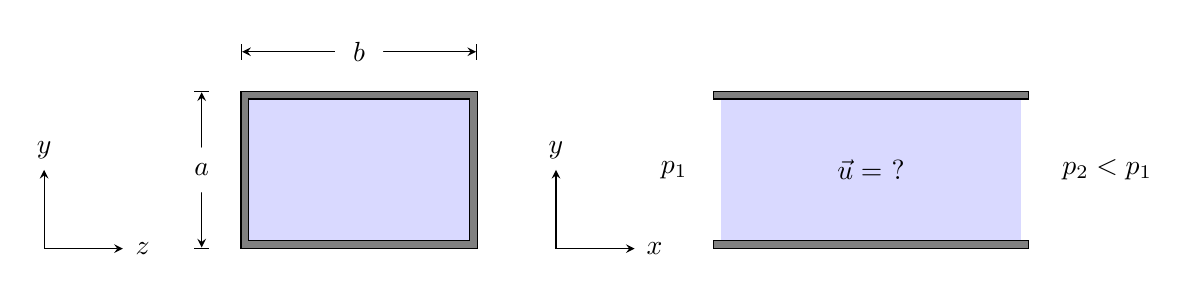
\begin{tikzpicture}
			% y-z plane
			\draw[<->, >=stealth] (-0.5,1) -- (-0.5,0) --(0.5,0);
			\node at (-0.5,1.25) {$y$};
			\node at (0.75,0) {$z$};
			
			% cross-section
			\draw[fill=gray] (2,0) rectangle (5,2);
			\draw[fill=blue!15!] (2.1,0.1) rectangle (4.9,1.9);
			
			% x-y plane
			\draw[<->, >=stealth] (6,1) -- (6,0) -- (7,0);
			\node at (6,1.25) {$y$};
			\node at (7.25,0) {$x$};
			
			% profile
			\path[fill=blue!15!] (8.1,0) rectangle (11.9,2);
			\draw[fill=gray] (8,0) rectangle (12,0.1);
			\draw[fill=gray] (8,2) rectangle (12,1.9);
			
			% velocity field
			\node at (10,1) {$\vec{u} =$ ?};
			
			% duct height
			\draw[|<->|, >=stealth] (1.5,0) -- (1.5,2);
			\node[circle, fill=white] at (1.5,1) {$a$};
			
			% duct width
			\draw[|<->|, >=stealth] (2,2.5) -- (5,2.5);
			\node[circle, fill=white] at (3.5,2.5) {$b$};
			
			% pressure
			\node at (7.5,1) {$p_1$};
			\node at (13,1) {$p_2 < p_1$};
		\end{tikzpicture}
		\caption{A schematic of the flow geometry}
		\label{fig:rect_duct}
	\end{figure}

    \subsection{Governing Equations}
    Using the provided assumptions, show that the Navier-Stokes equations reduce to
    \begin{align}
      \left(\frac{\partial^2}{\partial y^2} + \frac{\partial^2}{\partial z^2}\right) u(y,z) = \frac{1}{\mu}\frac{\partial p}{\partial x}.
    \end{align}
    \textbf{What are the boundary conditions?}
    
    % 2.1 Solution
    \begin{solution}
        % Problem 2.1 Solution
As before, let us start with the Navier-Stokes equations for an incompressible fluid.
\begin{align}
    \frac{\partial \vec{u}}{\partial t} + (\vec{u}\cdot\vec{\nabla})\vec{u} &= -\frac{1}{\rho}\vec{\nabla}p + \frac{\mu}{\rho}\nabla^2\vec{u}\\
    \vec{\nabla}\cdot\vec{u} &= 0
\end{align}
Note that we have already neglected the effect of any external body forces since the problem statement makes no mention of their importance. We already know from working through the problem on Couette flow that under steady flow conditions, $\partial \vec{u}/\partial t = 0$. Furthermore, since we are dealing with a one-component flow that is independent of $x$ (i.e. $u = u(y,z)$), then the nonlinear component vanishes.
\begin{equation}
    \vec{u}(\vec{\nabla}\cdot\vec{u}) = 0
\end{equation}
Thus, obeying the assumptions given in the problem statement essentially means our velocity profile must be of the form $\vec{u} = u(y,z)\ \hat{x}$, and the Navier-Stokes momentum equation simplifies as follows. 
\begin{equation}
    \boxed{\left(\frac{\partial^2}{\partial y^2} + \frac{\partial^2}{\partial z^2}\right)u(y,z) = \frac{1}{\mu}\frac{\partial p}{\partial x}}
    \label{snsmr}
\end{equation}
For this problem, no-slip boundary conditions imply that $u(y=0,z) = u(y=a,z) = 0$ and $u(y,z=0) = u(y,z=b) = 0$. 
    \end{solution}

    \subsection{Solving for $u$: Part 1}
    We have an inhomogenous, linear PDE on our hands.  Let's solve this using the method of eigenfunction expansions.  We know that with the current boundary conditions, the homogenous solution to our equation has eigenfunctions that are sines. Hence, let's assume a solution of the form
    \begin{align}
      u\left(y, z\right) = \sum_{n=1}^{\infty}{\beta_{n}\left(z\right)\sin\left(\frac{n\pi}{a}y\right)}.
    \end{align}
    Substitute this ansatz into the governing PDE and show that the unknown coefficients, $\beta_{n}\left(z\right)$, are governed by the following inhomogenous ODE.
    \begin{align}
        \beta_{n}^{\prime\prime} - \gamma_{n}^{2}\beta_{n} = q_{n}
        \label{eq:betan}
    \end{align}
    Here, $\left(\cdot\right)^{\prime}$ denotes $d/dz$, $\gamma_n$ is the eigenvalue, and $q_n$ and $Q$ are defined as follows.
    \begin{align}
        \gamma_n &= \frac{n \pi}{a}\\
        q_{n} &= \dfrac{2}{a}\int_{0}^{a}{Q\sin\left(\gamma_{n}y\right)\ \mathrm{d}y}\\
        Q &= \frac{1}{\mu}\frac{\partial p}{\partial x}
    \end{align}

    \subsubsection{Some Specific Details}
    Here is a breakdown of the required steps.
    \begin{enumerate}
      \item First show that after plugging the assumed form into the governing PDE the resulting expression is 
      \begin{align}
        \sum_{n=1}^{\infty}{\beta_{n}^{\prime\prime}\sin\left(\dfrac{n\pi}{a}y\right)} -
\sum_{n=1}^{\infty}{\beta_{n}\left(\dfrac{n\pi}{a}\right)^{2}\sin\left(\dfrac{n\pi}{a}y\right)} = Q.
      \end{align}
      \item Next, multiply by $\sin\left(\dfrac{m\pi}{a}y\right)$ and integrate over $y$.
      \begin{align}
        &\int_{0}^{a}{\sum_{n=1}^{\infty}{\beta_{n}^{\prime\prime}\sin\left(\dfrac{n\pi}{a}y\right)\sin\left(\dfrac{m\pi}{a}y\right)}
\ \mathrm{d}y} -
\int_{0}^{a}{\sum_{n=1}^{\infty}{\beta_{n}\left(\dfrac{n\pi}{a}\right)^{2}\sin\left(\dfrac{n\pi}{a}y\right)\sin\left(\dfrac{m\pi}{a}y\right)}
\ \mathrm{d}y} = \nonumber \\
        &\hspace{2.0em}\int_{0}^{a}{Q\sin\left(\dfrac{m\pi}{a}y\right) \ \mathrm{d}y}.
      \end{align}
      \item That's a pretty big mess.  Now, we use a beautiful result:  the orthogonality of sines:
        \begin{align}
          \int_{0}^{a}{\sin\left(\dfrac{n\pi}{a}y\right)\sin\left(\dfrac{m\pi}{a}y\right) \ \mathrm{d}y} = 
          \left\{
            \begin{array}{ll}
              0            \qquad n \neq m \\
              \dfrac{a}{2} \qquad n = m
            \end{array}
          \right.
        \end{align}
        The main point here is that every single term in the infinite sum is zero \textit{except} for the term where $n=m$.
      \item The final result is 
        \begin{align}
          \beta_{n}^{\prime\prime} - \gamma_{n}^{2}\beta_{n} = \dfrac{2}{a}\int_{0}^{a}{Q\sin\left(\gamma_{n}y\right) \ \mathrm{d}y}
        \end{align}
    \end{enumerate}

    \textbf{What are the boundary conditions on $\beta_{n}$}?
    
    % 2.2 Solution
    \begin{solution}
        % Problem 2.2 Solution
To proceed, we assume a solution of the form
\begin{equation}
    u(y,z) = \sum_{n=1}^{\infty} \beta_n(z) \sin\left(\frac{n \pi y}{a}\right).
\end{equation}
Substituting this into equation (\ref{snsmr}) yields the following.
\begin{equation}
    -\sum_{n=1}^{\infty} \beta_n(z) \left(\frac{n \pi}{a}\right)^2 \sin\left(\frac{n \pi y}{a}\right) + \sum_{n=1}^{\infty} \beta_n''(z) \sin\left(\frac{n \pi y}{a}\right) = \frac{1}{\mu}\frac{\partial p}{\partial x}
\end{equation}
We now exploit the orthogonality of the basis functions by multiplying through by $\sin(\gamma_m y)$ and integrating over $y$. We will examine each of the three terms individually to make the bookkeeping go smoothly.
\begin{align}
    \int_{0}^{a} \sum_{n=1}^{\infty} \beta_n''(z) \sin\left(\frac{n \pi y}{a}\right) \sin\left(\frac{m \pi y}{a}\right)\ dy &= \beta_m''(z) \frac{a}{2}\\
    \int_{0}^{a} \sum_{n=1}^{\infty} \beta_n(z) \left(\frac{n \pi}{a}\right)^2 \sin\left(\frac{n \pi y}{a}\right) \sin\left(\frac{m \pi y}{a}\right)\ dy &= \beta_m(z) \left(\frac{m \pi}{a}\right)^2 \frac{a}{2}\\
    \int_{0}^{a} \frac{1}{\mu}\frac{\partial p}{\partial x} \sin\left(\frac{m \pi y}{a}\right)\ dy &= \int_{0}^{a} Q \sin\left(\frac{m \pi y}{a}\right)\ dy
\end{align}
Putting everything together allows to obtain an ordinary differential equation for the coefficients, $\beta_m(z)$.
\begin{equation}
    \beta_m''(z) - \beta_m(z) \left(\frac{m \pi}{a}\right)^2 = \frac{2}{a}\int_{0}^{a} Q \sin\left(\frac{m \pi y}{a}\right)
\end{equation}
Recall that $\gamma_m = m\pi/a$, and if we define
\begin{equation}
    q_m = \frac{2}{a}\int_{0}^{a} Q \sin\left(\frac{m \pi y}{a}\right),
\end{equation}
we may rewrite the previous ODE as
\begin{equation}
    \beta_m'' - \gamma_m^2 \beta_m = q_m.
\end{equation}
At this point, we can exchange the index $m$ for $n$ such that our end result can be written as follows.
\begin{equation}
    \boxed{\beta_n'' - \gamma_n^2 \beta_n = q_n}
    \label{odebeta}
\end{equation}
Recall that we are working with no-slip boundary conditions on all sides. Thus, the boundary conditions on $\beta_n$ must be $\beta_n(z=0) = \beta_n(z=b) = 0$.
    \end{solution}

    \subsection{Solving for $\beta_{n}$: The Homogeneous Part}
    To solve for $\beta_{n}$, we first need to solve the homogeneous equation,
    \begin{align}
      \beta_{n}^{\prime\prime} - \gamma_{n}^{2}\beta_{n} = 0.
    \end{align}
    Show that the homogeneous solution is 
    \begin{align}
      \beta_{n}^{H} = c_{1}w_{1} + c_{2}w_{2}
    \end{align}
    where $w_{1} = \sinh\left(\gamma_{n}z\right)$ and $w_{2} = \cosh\left(\gamma_{n}z\right)$ are the two linearly independent solutions.
    
    % 2.3 Solution
    \begin{solution}
        % Problem 2.3 Solution
We now turn our attention to solving equation (\ref{odebeta}). To do this, we first solve the homogeneous equation, 
\begin{equation}
    \beta_n'' - \gamma_n^2 \beta_n = 0,
    \label{odebeta}
\end{equation}
by assuming a solution of the form $\beta_n(z) = e^{\lambda_n z}$. Substituting our ansatz into equation (\ref{odebeta}) yields the characteristic polynomial.
\begin{equation}
    \lambda_n^2 e^{\lambda_n z} - \gamma_n^2 e^{\lambda_n z} = 0 \implies \lambda_n = \pm\gamma_n
\end{equation}
Hence, the general solution to the homogeneous problem can be written as follows.
\begin{align}
    \beta_n^H(z) &= a e^{-\lambda_n z} + b e^{\lambda_n z}\\
    &= a e^{-\gamma_n z} + b e^{\gamma_n z}
\end{align}
However, we may also write the general solution in terms of a different set of linearly independent functions. Recall that the hyperbolic sine and cosine functions are linear combinations of the exponential functions, $e^x$ and $e^{-x}$.
\begin{align}
    \sinh(x) &= \frac{1}{2}\left(e^{x} - e^{-x}\right)\\
    \cosh(x) &= \frac{1}{2}\left(e^{x} + e^{-x}\right)
\end{align}
Hence, if we let $x = \gamma_n z$, we may, without loss of generality, write the general solution to the homogeneous problem as 
\begin{equation}
    \boxed{\beta_n^H(z) = c_1 \sinh(\gamma_n z) + c_2 \cosh(\gamma_n z).}
\end{equation}
    \end{solution}

    \subsection{Solving the Inhomogeneous Part}
    You can use the method of variation of parameters to solve the inhomogeneous equation.  Let 
    \begin{align}
        \beta_{n}\left(z\right) = v_{1}\left(z\right)w_{1}\left(z\right) + v_{2}\left(z\right)w_{2}\left(z\right),
        \label{eq:var_param}
    \end{align}
    where $v_{1}\left(z\right)$ and $v_{2}\left(z\right)$ are the coefficients (parameters) to be varied.  Now, \emph{assume} that 
    \begin{align}
        w_{1}v_{1}^{\prime} + w_{2}v_{2}^{\prime} = 0.
        \label{eq:var_const}
    \end{align}
    Substituting \eqref{eq:var_param} into~\eqref{eq:betan} and using~\eqref{eq:var_const} yields two equations for
$v_{1}^{\prime}$ and $v_{2}^{\prime}$.
    \begin{align}
      w_{1}v_{1}^{\prime} + w_{2}v_{2}^{\prime} &= 0 \\
      w_{1}^{\prime}v_{1}^{\prime} + w_{2}^{\prime}v_{2}^{\prime} &= q_{n}
    \end{align}
    Show that 
    \begin{align}
      v_{1} &= \frac{q_{n}}{\gamma_{n}^{2}}\sinh\left(\gamma_{n}z\right) + \alpha_{1} \\
      v_{2} &= -\frac{q_{n}}{\gamma_{n}^{2}}\cosh\left(\gamma_{n}z\right) + \alpha_{2} 
    \end{align}
    where $\alpha_{1}$ and $\alpha_{2}$ are constants of integration.

    Finally, show that 
    \begin{align}
      \beta_{n}\left(z\right) &= C_{n} 
        \left[-\sinh\left(\gamma_{n}b\right) + \sinh\left(\gamma_{n}z\right) - 
          \left(\sinh\left(\gamma_{n}z\right)\cosh\left(\gamma_{n}b\right) - 
            \cosh\left(\gamma_{n}z\right)\sinh\left(\gamma_{n}b\right)\right)\right] \\
      &=  C_{n}
           \left[\sinh\left(\gamma_{n}z\right) - \sinh\left(\gamma_{n}b\right) - 
            \sinh\left(\gamma_{n}\left(z-b\right)\right)\right] \label{eq:beta-cn}\\
      &= 2C_{n}\sinh\left(\dfrac{\gamma_{n}}{2}\left(z-b\right)\right) 
           \left[\cosh\left(\dfrac{\gamma_{n}}{2}\left(z+b\right)\right) - 
             \cosh\left(\dfrac{\gamma_{n}}{2}\left(z-b\right)\right)\right].
    \end{align}
    where 
    \begin{align}
      C_{n} = \frac{q_{n}}{\gamma_{n}^{2}\sinh\left(\gamma_{n}b\right)}. 
    \end{align}
    
    % 2.4 Solution
    \begin{solution}
        % Problem 2.4 Solution
Following the procedure outlined in the problem statement, we will start by substituting equation \eqref{eq:var_param} into equation \eqref{eq:betan}.
\begin{equation}
    \beta_n' = v_1 w_1' + v_1' w_1 + v_2 w_2' + v_2' w_2
\end{equation}
If we assume that $w_1 v_1' + w_2 v_2' = 0$, the previous equation simplifies as follows.
\begin{equation}
    \beta_n' = v_1 w_1' + v_2 w_2'
    \label{eq:betan-prime}
\end{equation}
From here, we can differentiate equation \eqref{eq:betan-prime} to obtain
\begin{equation}
    \beta_n'' = v_1' w_1' + v_1 w_1'' + v_2' w_2' + v_2 w_2''.
\end{equation}
Putting all of this together yields the following.
\begin{equation}
    v_1' w_1' + v_1 w_1'' + v_2' w_2' + v_2 w_2'' - \gamma_n^2(v_1 w_1 + v_2 w_2) = q_n
    \label{eq:beta-var-param_expanded}
\end{equation}
Now, recall that we have defined $w_1 = \sinh(\gamma_n z)$ and $w_2 = \cosh(\gamma_n z)$. Therefore, $w_1'' = \gamma_n^2 w_1$ and $w_2'' = \gamma_n^2 w_2$, and equation \eqref{eq:beta-var-param_expanded} can be rewritten as follows.
\begin{equation}
    v_1' w_1' + v_2' w_2' + \gamma_n^2(v_1 w_1 + v_2 w_2) - \gamma_n^2(v_1 w_1 + v_2 w_2) = q_n
\end{equation}
Notice that several of the terms cancel, leaving us with
\begin{equation}
    v_1' w_1' + v_2' w_2' = q_n.
\end{equation}
We now have two equations for $v_1'$ and $v_2'$.
\begin{align}
    w_1 v_1' + w_2 v_2' &= 0\\
    v_1' w_1' + v_2' w_2' &= q_n
\end{align}
These can be written explicitly in terms of $\sinh(\gamma_n z)$ and $\cosh(\gamma_n z)$.
\begin{align}
    \sinh(\gamma_n z) v_1' + \cosh(\gamma_n z) v_2' &= 0\\
    \gamma_n \cosh(\gamma_n z) v_1' + \gamma_n \sinh(\gamma_n z) v_2' &= 0 \label{eq:odev1v2}
\end{align}
To proceed, we will use the first equation to isolate $v_2'$.
\begin{equation}
    v_2' = -\frac{\sinh(\gamma_n z)}{\cosh(\gamma_n z)}v_1'
    \label{eq:v2prime}
\end{equation}
From here, we can substitute equation \eqref{eq:v2prime} into equation \eqref{eq:odev1v2} to obtain an expression for $v_1'$.
\begin{align}
    \gamma_n \cosh(\gamma_n z) v_1' + \gamma_n \sinh(\gamma_n z) \left[-\frac{\sinh(\gamma_n z)}{\cosh(\gamma_n z)} v_1'\right] &= q_n\\
    \gamma_n v_1' \left[\cosh(\gamma_n z) - \frac{\sinh^2(\gamma_n z)}{\cosh(\gamma_n z)}\right] &= q_n\\
    \frac{\gamma_n v_1'}{\cosh(\gamma_n z)} &= q_n\\
    v_1' &= \frac{q_n}{\gamma_n}\cosh(\gamma_n z) \label{eq:v1prime}
\end{align}
Integrating equation \eqref{eq:v1prime} yields
\begin{equation}
    \boxed{v_1 = \frac{q_n}{\gamma_n^2} \sinh(\gamma_n z) + \alpha_1,}
\end{equation}
where $\alpha_1$ is a constant of integration. Likewise, we can now use equation \eqref{eq:v1prime} to obtain a solution for $v_2$.
\begin{align}
    v_2' &= -\frac{\sinh(\gamma_n z)}{\cosh(\gamma_n z)}\left[\frac{q_n}{\gamma_n}\cosh(\gamma_n z)\right]\nonumber\\
    &= -\frac{q_n}{\gamma_n} \sinh(\gamma_n z) \label{eq:v2prime-explicit}
\end{align}
Integrating equation \eqref{eq:v2prime-explicit} yields
\begin{equation}
    \boxed{v_2 = -\frac{q_n}{\gamma_n^2} \cosh(\gamma_n z) + \alpha_2,}
\end{equation}
where $\alpha_2$ is a second constant of integration. Putting all of this together allows us to write a general solution for $\beta_n(z)$.
\begin{align}
    \beta_n(z) &= v_1 w_1 + v_2 w_2\nonumber\\
    &= \left[\frac{q_n}{\gamma_n^2}\sinh(\gamma_n z) + \alpha_1\right]\sinh(\gamma_n z) + \left[\alpha_2 - \frac{q_n}{\gamma_n^2}\cosh(\gamma_n z)\right]\cosh(\gamma_n z) \label{eq:beta-gen-sol}
\end{align}
We can now impose the boundary conditions to determine the constants of integration, $\alpha_1$ and $\alpha_2$.
\begin{equation}
    \beta_n(z=0) = 0 = -\frac{q_n}{\gamma_n^2} + \alpha_2
    \implies 
    \alpha_2 = \frac{q_n}{\gamma_n^2}
\end{equation}
Obtaining an expression for $\alpha_1$ involves more algebra, but the idea is the same.
\begin{align}
    \beta_n(z=b) = 0 &= \left[\frac{q_n}{\gamma_n^2}\sinh(\gamma_n b) + \alpha_1\right]\sinh(\gamma_n b) + \left[\frac{q_n}{\gamma_n^2} - \frac{q_n}{\gamma_n^2}\cosh(\gamma_n b)\right]\cosh(\gamma_n b)\\
    \alpha_1 &= \frac{q_n}{\gamma_n^2 \sinh(\gamma_n b)}\left[\cosh^2(\gamma_n b) - \sinh^2(\gamma_n b) - \cosh(\gamma_n b)\right]\\
    \alpha_1 &= \frac{q_n}{\gamma_n^2 \sinh(\gamma_n b)}\left[1 - \cosh(\gamma_n b)\right]
\end{align}
Putting all of this together allows us to rewrite \eqref{eq:beta-gen-sol} as follows.
\begin{align}
    \beta_n(z) &= \frac{q_n}{\gamma_n^2}\left[\sinh(\gamma_n z) + \frac{1 - \cosh(\gamma_n b)}{\sinh(\gamma_n b)}\right]\sinh(\gamma_n z) + \frac{q_n}{\gamma_n^2}\left[1 - \cosh(\gamma_n z)\right]\cosh(\gamma_n z)\nonumber\\
    &= \frac{q_n}{\gamma_n^2} \left[\sinh^2(\gamma_n z) + \frac{\sinh(\gamma_n z) - \cosh(\gamma_n b)\sinh(\gamma_n z)}{\sinh(\gamma_n b)} + \cosh(\gamma_n z) - \cosh^2(\gamma_n z)\right]\nonumber\\
    &= \frac{q_n}{\gamma_n^2 \sinh(\gamma_n b)}\left[\sinh(\gamma_n z) - \sinh(\gamma_n b) - \cosh(\gamma_n b)\sinh(\gamma_n z) + \cosh(\gamma_n z)\sinh(\gamma_n b)\right]\nonumber\\
    &= \frac{q_n}{\gamma_n^2 \sinh(\gamma_n b)}\left[\sinh(\gamma_n z) - \sinh(\gamma_n b) -\sinh(\gamma_n(z-b))\right] \label{eq:beta-cn-2}
\end{align}
Notice that if we let 
\begin{equation}
    C_n = \frac{q_n}{\gamma_n^2 \sinh(\gamma_n b)},
\end{equation}
equations \eqref{eq:beta-cn} and \eqref{eq:beta-cn-2} agree. Thus, we may write the end result as 
\begin{equation}
    \boxed{\beta_n(z) = 2C_n \sinh\left(\frac{\gamma_n}{2}(z-b)\right)\left[\cosh\left(\frac{\gamma_n}{2}(z+b)\right) - \cosh\left(\frac{\gamma_n}{2}(z-b)\right)\right].}
\end{equation}
    \end{solution}

    \subsection{The Velocity Field}
    Put everything together to show that the velocity profile can be written as follows.
    \begin{align}
      u\left(y,z\right) = \sum_{n=1}^{\infty}{2C_{n} 
        \sinh\left(\dfrac{\gamma_{n}}{2}\left(z-b\right)\right)\left[\cosh\left(\dfrac{\gamma_{n}}{2}\left(z+b\right)\right) - 
          \cosh\left(\dfrac{\gamma_{n}}{2}\left(z-b\right)\right)\right]\sin\left(\gamma_{n}y\right)}
    \end{align}
    A good sanity check is to make sure the boundary conditions are satisfied by this solution.

    \subsubsection{Other Thoughts}
    There are a variety of things that can be computed and inspected from here.  For example:
    \begin{itemize}
      \item Calculate the vorticity and streamlines.  Any surprises here?
      \item How does the solution change if you have different boundary conditions?
        \begin{itemize}
          \item Neumann boundary conditions on each surface 
          \item Dirichlet boundary conditions on all surfaces \emph{except} at $y=a$ for which we have a Neumann condition. (This would be like fluid flowing through an open channel.)
        \end{itemize}
    \end{itemize}
    \textbf{Note:}  You are not required to compute any of these for this assignment!
    
    % 2.5 Solution
    \begin{solution}
        % Problem 2.5 Solution
Recall that our analysis has assumed a product solution of the form 
\begin{equation}
    u(y,z) = \sum_{n=0}^{\infty} \beta_n(z) \sin\left(\frac{n \pi y}{a}\right). 
    \label{eq:u-ansatz}
\end{equation}
Substituting our solution for $\beta_n(z)$ into equation \eqref{eq:u-ansatz} yields the end result.
\begin{equation}
    \boxed{u(y,z) = \sum_{n=0}^{\infty} 2C_n \sinh\left(\frac{\gamma_n}{2}(z-b)\right)\left[\cosh\left(\frac{\gamma_n}{2}(z+b)\right) - \cosh\left(\frac{\gamma_n}{2}(z-b)\right)\right] \sin(\gamma_n y)}
\end{equation}
From here, we can obtain other relevant quantities, such as the vorticity and streamlines. Remember that the vorticity is the curl of the velocity field.
\begin{align}
    \vec{\omega} &= \vec{\nabla}\times\vec{u}\\
    &= \left(\frac{\partial}{\partial x}\hat{x} + \frac{\partial}{\partial y}\hat{y} + \frac{\partial}{\partial z}\hat{z}\right) \times u(y,z)\hat{x}\\
    &= \frac{\partial u}{\partial x} (\hat{x}\times\hat{x}) + \frac{\partial u}{\partial y} (\hat{y}\times\hat{x}) + \frac{\partial u}{\partial z} (\hat{z}\times\hat{x})\\
    &= \frac{\partial u}{\partial z}\hat{y} - \frac{\partial u}{\partial y}\hat{z}\\
    &= \beta_n'(z) \sin(\gamma_n y)\ \hat{y} - \gamma_n \beta_n(z) \cos(\gamma_n y)\ \hat{z}
\end{align}
Substituting in the explicit form of $\beta_n(z)$ and $\beta_n'(z)$ and simplifying our expression gives the following result.
\begin{align}
    \vec{\omega} = &\gamma_n C_n \left[\cosh(\gamma_n z) - \cosh(\gamma_n(z-b))\right]\sin(\gamma_n y)\ \hat{y} \dots\nonumber\\
    &- 2 \gamma_n C_n \sinh\left(\frac{\gamma_n}{2}(z-b)\right)\left[\cosh\left(\frac{\gamma_n}{2}(z+b)\right) - \cosh\left(\frac{\gamma_n}{2}(z-b)\right)\right] \cos(\gamma_n y)\ \hat{z}
\end{align}
    \end{solution}

  \subsection{Visualization}
  Now that we have an explicit formula for the velocity field, we can visualize it.  Try to make the following plots:
  \begin{itemize}
    \item Plot $u\left(y,z=z^{*}\right)$ at a few values of $z^{*}$ (perhaps near the boundary, $1/4$ of the channel width, and
at half the channel width).
    \item Plot $u\left(y=y^{*},z\right)$ at a few values of $y^{*}$ (perhaps near the boundary, $1/4$ of the channel height, and
at half the channel height).
    \item Make a surface plot of $u\left(y,z\right)$.
  \end{itemize}
  
    % 2.6 Solution
    \begin{solution}
        % Problem 2.6 Solution
% Plots for each value of y^* and z^*
\begin{figure}[H]
    \centering
    \includegraphics[scale=0.75]{figures/rect-duct_ystar.pdf}
    \caption{A plot of the velocity profiles at several values of $y^*$}
    \label{fig:ystar}
\end{figure}

\begin{figure}[H]
    \centering
    \includegraphics[scale=0.75]{figures/rect-duct_zstar.pdf}
    \caption{A plot of the velocity profiles at several values of $z^*$}
    \label{fig:zstar}
\end{figure}

% Surface plot of the velocity field
\begin{figure}[H]
    \centering
    \includegraphics[scale=0.85]{figures/rect-duct_velocity-profile.pdf}
    \caption{A surface plot of the velocity profile for flow in a rectangular duct}
\end{figure}
    \end{solution}
    \pagebreak

  \section{Problem 3: The Finite Element Method}

  Consider the steady one-dimensional advection-diffusion-reaction equation,
  \begin{align}
    a\partial_{x}u -\lambda u - k\partial_{x}^{2}u = f, \qquad x\in\left(0, 1\right)
    \label{eq:adv-diff-rxn}
  \end{align}
  with boundary conditions 
  \begin{align}
    u\left(0\right) = u_{0}, \quad -k\partial_{x}u\left(1\right) = b_{1}.
    \label{eq:adr_bcs}
  \end{align}
  In~\eqref{eq:adv-diff-rxn}, $a$ is the constant advection speed, $\lambda > 0$ is the constant reaction coefficient, and $k>0$ 
  is the constant diffusion coefficient.  

  \subsection{Weak Form}
  Write the weak form corresponding to the strong form~\eqref{eq:adv-diff-rxn}.  Be sure to specify all function spaces. Don't forget to include any boundary terms.

  \begin{solution}
    Equation \eqref{eq:adv-diff-rxn} denotes the strong form $\textbf{S}$. Multiplying $\textbf{S}$ by a test function, $w(x)$, and integrating over the domain yields the following.
    \begin{gather}
        \int_0^1 w\left(a\partial_{x}u -\lambda u - k\partial_{x}^{2}u\right) dx = \int_0^1 wf dx \\
        \int_0^1 wa\partial_{x}u dx -\int_0^1 w\lambda u dx - \int_0^1 wk\partial_{x}^{2}u dx = \int_0^1 wf dx
    \end{gather}
    Use integration by parts on the third term on the LHS, we have
    \begin{equation}
        \int_0^1 wk\partial_{x}^{2}u dx = k \left( w \partial_{x}u \Big|_0^1 - \int_0^1 \partial_{x}w \partial_{x}u dx \right)
    \end{equation}
    Set $w(0) = 0$, and we know that $k\partial_{x}u(1) = -b_1$, substitute Eq.(102) into Eq.(101), we have
    \begin{gather}
        \int_0^1 wa\partial_{x}u dx -\int_0^1 w\lambda u dx - w(1)k\partial_{x}u(1) + w(0)k\partial_{x}u(0) + \int_0^1 k\partial_{x}w \partial_{x}u dx = \int_0^1 wf dx \notag \\
        \int_0^1 wa\partial_{x}u dx -\int_0^1 w\lambda u dx - w(1)b_1 + \int_0^1 k\partial_{x}w \partial_{x}u dx = \int_0^1 wf dx
    \end{gather}
    
    Function spaces: $S = \left \{ u \Big| u \in H^1, u(0) = u_0 \right \}$ and $V = \left \{ v \Big| v \in H^1, v(0) = 0 \right \}$.

	\begin{tcolorbox}
	The weak form: Find $u \in S$, s.t. $\forall w \in V$, $u \in V$, 
	\begin{equation*}
	a\int_0^1 w\partial_{x}u dx - \lambda \int_0^1 w u dx + k \int_0^1 \partial_{x}w \partial_{x}u dx = \int_0^1 wf dx + w(1)b_1
	\end{equation*}
	
	\end{tcolorbox}    
    
   

\end{solution}

  \subsection{Galerkin Statement}
  From the weak form, write the Galerkin statement.  Again, specify all function spaces.
  
  \begin{solution}
	Function spaces: $S = \left \{ u \Big| u \in H^1, u(0) = u_0 \right \}$ and $V = \left \{ v \Big| v \in H^1, v(0) = 0 \right \}$. Let $u^h = v^h + g^h$ where $g^h(0)=u_0$, we have
	\begin{gather}
		a\int_0^1 w^h\partial_{x}(v^h + g^h) dx - \lambda \int_0^1 w^h (v^h + g^h) dx + k \int_0^1 \partial_{x}w^h \partial_{x}(v^h + g^h) dx \notag \\
		= \int_0^1 w^h f dx + w^{h}(1)b_1
	\end{gather}
	
	\begin{tcolorbox}
		The Galerkin statement: Find $u^h \in S^h \subset S$, s.t. $\forall w^h \in V^h \subset V$, $u^h \in V^h$, 
		\begin{gather*}
			a\int_0^1 w^h\partial_{x}v^h dx - \lambda \int_0^1 w^h v^h dx + k \int_0^1 \partial_{x}w^h \partial_{x}v^h dx \notag \\
		= \int_0^1 w^h f dx + w^{h}(1)b_1 - a\int_0^1 w^h\partial_{x}g^h dx + \lambda \int_0^1 w^h g^h dx - k \int_0^1 \partial_{x}w^h \partial_{x}g^h dx
		\end{gather*}
		the weak form is satisfied. 	
	\end{tcolorbox}
	
\end{solution}

  \subsection{Finite Element Discretization}
  Introduce the finite element basis and arrive at a linear algebra problem.  Clearly define the form of all resulting matrices.  You may write everything in terms of the basis functions (i.e. there is no need to directly compute the entries of the matrices).

  \begin{solution}
	Since $w^h, v^h \in V^h$, let 
	\begin{align}
		w^h &= \sum_{A=1}^n w_A N_A(x) \\
		v^h &= \sum_{B=1}^n u_B N_B(x) \\
		g^h &= u_0 N_{n+1}(x) \\
		u^h &= v^h + g^h = \sum_{B=1}^n u_B N_B(x) + u_0 N_{n+1}(x)
	\end{align}
	where $N_A(0) = 0, N_B (0) = 0, N_{n+1}(0) = 1$. Substitute Eq.(105-108) into the Galerkin statement, we have
	\begin{gather}
			a\int_0^1 \left(\sum_{A=1}^n w_A N_A(x)\right) \partial_{x}\left( \sum_{B=1}^n u_B N_B(x) \right) dx - \lambda \int_0^1 \left(\sum_{A=1}^n w_A N_A(x)\right) \left( \sum_{B=1}^n u_B N_B(x) \right) dx \notag \\
			+ k \int_0^1 \partial_{x}\left(\sum_{A=1}^n w_A N_A(x)\right) \partial_{x}\left( \sum_{B=1}^n u_B N_B(x) \right) dx \notag \\
		= \int_0^1 \left(\sum_{A=1}^n w_A N_A(x)\right) f dx + \left(\sum_{A=1}^n w_A N_A(1)\right)b_1 - a\int_0^1 \left(\sum_{A=1}^n w_A N_A(x)\right) \partial_{x}\left( u_0 N_{n+1}(x) \right) dx \notag \\
		+ \lambda \int_0^1 \left(\sum_{A=1}^n w_A N_A(x)\right) \left( u_0 N_{n+1}(x) \right) dx - k \int_0^1 \partial_{x}\left(\sum_{A=1}^n w_A N_A(x)\right) \partial_{x}\left( u_0 N_{n+1}(x) \right) dx
	\end{gather}
	Denote the basis functions $N_A(x)$ and $N_B(x)$ to be nonnegative, by the Fubini Theorem, we can simplify Eq.(109) into
	\begin{align}
		\sum_{A=1}^n w_A & \left( a\int_0^1 N_A(x) \partial_{x} \left( \sum_{B=1}^n u_B N_B(x) \right) dx - \lambda \int_0^1 N_A(x) \left( \sum_{B=1}^n u_B N_B(x) \right) dx \notag \right. \notag \\
		&+ k \int_0^1 \partial_{x}\left(N_A(x)\right) \partial_{x}\left( \sum_{B=1}^n u_B N_B(x) \right) dx - \int_0^1 f N_A dx - N_A(1) b_1 \notag \\
		&+ a \int_0^1 N_A(x) \partial_{x}\left( u_0 N_{n+1}(x) \right) dx - \lambda u_0 \int_0^1 N_A(x) N_{n+1}(x) dx \notag \\
		&\left. + k u_0 \int_0^1 \partial_{x}(N_A(x)) \partial_{x}(N_{n+1}(x)) dx \right) = 0
	\end{align}
	To satisfy Eq.(110), the terms in the bracket must be zero:
	\begin{gather}
		a\int_0^1 N_A(x) \partial_{x} \left( \sum_{B=1}^n u_B N_B(x) \right) dx - \lambda \int_0^1 N_A(x) \left( \sum_{B=1}^n u_B N_B(x) \right) dx \notag \\
		+ k \int_0^1 \partial_{x}\left(N_A(x)\right) \partial_{x}\left( \sum_{B=1}^n u_B N_B(x) \right) dx - \int_0^1 f N_A dx - N_A(1) b_1 \notag \\
		+ a \int_0^1 N_A(x) \partial_{x}\left( u_0 N_{n+1}(x) \right) dx - \lambda u_0 \int_0^1 N_A(x) N_{n+1}(x) dx \notag \\
		+ k u_0 \int_0^1 \partial_{x}(N_A(x)) \partial_{x}(N_{n+1}(x)) dx = 0
	\end{gather}
	By applying the Fubini Theorem again, we have
	\begin{gather}
	    \sum_{B=1}^n a\int_0^1 N_A(x) \partial_{x} \left( u_B N_B(x) \right) dx - \sum_{B=1}^n \lambda \int_0^1 N_A(x) \left( u_B N_B(x) \right) dx \notag \\
	    + \sum_{B=1}^n k \int_0^1 \partial_{x}\left(N_A(x)\right) \partial_{x}\left( u_B N_B(x) \right) dx \notag \\
	    = \int_0^1 f N_A dx + N_A(1) b_1 - a \int_0^1 N_A(x) \partial_{x}\left( u_0 N_{n+1}(x) \right) dx \notag \\
	    + \lambda u_0 \int_0^1 N_A(x) N_{n+1}(x) - k u_0 \int_0^1 \partial_{x}(N_A(x)) \partial_{x}(N_{n+1}(x)) dx
	\end{gather}
	Denote the series and integrals in Eq.(112) as
	\begin{align}
	    \sum_{B=1}^n A_{AB} u_B &= \sum_{B=1}^n a\int_0^1 N_A(x) \partial_{x} \left( u_B N_B(x) \right) dx \\
	    \sum_{B=1}^n \Lambda_{AB} u_B &= \sum_{B=1}^n \lambda \int_0^1 N_A(x) \left( u_B N_B(x) \right) dx \\
	    \sum_{B=1}^n K_{AB} u_B &= \sum_{B=1}^n k \int_0^1 \partial_{x}\left(N_A(x)\right) \partial_{x}\left( u_B N_B(x) \right) dx \\
	    F_A &= \int_0^1 f N_A dx + N_A(1) b_1 - a \int_0^1 N_A(x) \partial_{x}\left( u_0 N_{n+1}(x) \right) dx \notag \\
	    &+ \lambda u_0 \int_0^1 N_A(x) N_{n+1}(x) - k u_0 \int_0^1 \partial_{x}(N_A(x)) \partial_{x}(N_{n+1}(x)) dx
	\end{align}
	where
	\begin{align}
	    A_{AB} &= \int_0^1 N_A(x) \partial_{x} \left( N_B(x) \right) dx \\
	    \Lambda_{AB} &= \int_0^1 N_A(x) \left( N_B(x) \right) dx \\
	    K_{AB} &= \int_0^1 \partial_{x}\left(N_A(x)\right) \partial_{x}\left( N_B(x) \right) dx
	\end{align}
		
		
	\begin{tcolorbox}
		We reach the linear algebra problem: Solve for
		\begin{equation*}
		    \sum_{B=1}^n a A_{AB}u_B - \sum_{B=1}^n \lambda \Lambda_{AB}u_B	+ \sum_{B=1}^n k K_{AB}u_B = F_A, A = 1, \cdots, n
		\end{equation*}
		where $A_{AB}, \Lambda_{AB}, K_{AB}, F_A$ are denoted in Eq.(116-119).
	\end{tcolorbox}
	
\end{solution}
  \pagebreak
  
  \section{Problem 4: Implementation}
  We wish to use the finite element method to solve 
  \begin{align}
    - \partial_{x}^{2} u = f\lr{x}, \qquad x \in \lr{0, 1} \\
    -\partial_{x}u\lr{0} = \mathcal{h}, \quad u\lr{1} = \mathcal{g}
  \end{align}
  for $u\lr{x}$ where $f\lr{x}$ is a known forcing function and $\mathcal{g}$ and $\mathcal{h}$ are constant boundary data.

  Write a one-dimensional finite element code that uses piecewise linear finite elements to solve for $u\lr{x}$.  The
following specifications are required:
  \begin{itemize}
    \item The code should work for any constant $\mathcal{g}$ and $\mathcal{h}$ as well as arbitrary $f\lr{x}$.  These will be inputs to the
code.
    \item Other inputs should include the domain size.  You have some flexibility on how to do this.  For example, you may
pass in a fully-formed mesh if you wish.  Alternatively, you can require the user to specify the number of elements from
which your code can compute the uniform mesh size.
      \begin{itemize}
        \item \textbf{Note:} You may assume a uniform mesh.
      \end{itemize}
    \item The code \textbf{must} use the local point of view.  That is, loop over individual elements and perform the finite
element assembly operation to form the global stiffness matrix and force vector.
    \item Use Gaussian quadrature to perform the integrals.  Although not strictly necessary here, it will give you some
intuition for how things are actually done.
    \item You may use an external library to solve the resulting linear system.
    \item Use must use a compiled language such as \texttt{C}, \texttt{C++}, or (modern) Fortran.
    \item Try to submit your job on Odyssey!
  \end{itemize}

  Some other things you may want to consider are the following:
  \begin{itemize}
    \item Start simple.  A natural progression may be the following:
      \begin{itemize}
        \item Select $f = 0$, $g = 0$ and $h = 1$ to begin.  The exact solution will be $u = 1 - x$.
        \item Then make $g = 1$, $h = 1$, $f = 0$.  The exact solution will be $u = 2 - x$.
        \item Finally, try $g = 1$, $h = 1$, and $f = 1$.  The exact solution will be $u = 2 - x + \dfrac{1}{2}\lr{1 -
x^{2}}$.
        \item At this point, you will have some confidence in your code.  This is called code verification.  You can try more
complicated $f\lr{x}$ if you'd like to.
      \end{itemize}
    \item Organize your code into separate files.  Use a \texttt{Makefile} to do the linking.
      \begin{itemize}
        \item You may want to have files for the following:
          \begin{itemize}
            \item Quadrature routines 
            \item Stiffness matrix routines 
            \item Right-hand-size (RHS) routines
          \end{itemize}
        \item Feel free to consider other code designs.
      \end{itemize}
  \end{itemize}
  
    % Problem 4 Solution
    \begin{solution}
        \input{HW1_P4_Jonathan/HW1_P4.tex}
    \end{solution}
  
\end{document}
